%
% ****
\chapter{Performance \& Auswertung}
\label{chap:erg}
% ****
%
	Ziel dieser Arbeit ist es, auf Grundlage eines bereits bestehenden, neuronalen Netzes eine Anwendung des Reinforcement Learning zur Regelung dynamischer Systeme zu schaffen. Das neuronale Netz ist dabei kein konventionell erzeugtes Netz einer künstlichen Intelligenz, sondern beruht auf biologischen Forschungsergebnissen echter Lebensformen.\\
	Somit wurde zuerst eine Berechnungsgrundlage eines solchen Netzes geschaffen und implementiert. Dazu wurden verschiedene numerische Lösungsverfahren von Differenzialgleichungen verglichen und umgesetzt. Letztlich wird ein universeller Simulator geschaffen, welcher Informationen über die Nervenzellen und Synapsen erhält und entsprechend in der Lage ist, das gesamte Netz zu simulieren und Fire-Events auszugeben. Um die Performance des neuronalen Netzes durch den Simulator zu messen, wird eine Simulationsumgebung eingebunden und ein Lern-Algorithmus implementiert. In dieser Arbeit wird sich auf die Reinforcement Learning Methode RandomSearch konzentriert sowie auf die Optimierungsmethode durch Gewichten der entsprechenden Synapsen.

% ***
\section{Performance implementierter Algorithmen}
\label{sec:erg_performance}
% ***
	Schnelligkeit der Ausführung von Algorithmen und ganzen Skripten ist in dieser Anwendung von großer Relevanz. Da der Simulator von Grund auf darauf ausgerichtet wurde, später rechenintensive Simulationen von Parametern zu durchlaufen, wurde bereits in der Auswahl der zusätzlich genutzten Pakete darauf geachtet, dass diese performant und Ressourceneffizient implementiert wurden.\\
	Angefangen bei den Berechnungsmodulen in der Datei \texttt{lif.py} wird für komplexere mathematische Operationen die Erweiterung \texttt{NumPy} aus dem bekannten Python-Paket \texttt{SciPy} genutzt. Weiterhin werden Schleifen und If-Abfragen ohne Redundanzen und unnötige Befehle implementiert, um in der höheren Abstraktionsebene einen einwandfreien Aufruf zu garantieren. Nach erfolgreichen Tests der implementierten Funktionen wurde das Framework für den Simulator erstellt. Genutzte Pakete wie \texttt{matplotlib} oder \texttt{hickle} sind ebenfalls für ihre Schnelligkeit und einfache Handhabung ausgewählt worden. Des Weiteren können hier die bereits implementierten Funktionen zur Berechnung von Synapsenströmen und Membranpotentialen einfach importiert werden.\\
	Letztendlich ist die Ausführung des Suchalgorithmus RandomSearch sowie de Optimierung durch den Algorithmus Weights ausschlaggebend. Diese Algorithmen wurden im Laufe der Implementierung immer wieder optimiert und verbessert, sodass eine zuverlässige Simulation mit effizienten Laufzeiten möglich wird. Bei festen Simulationszeiten werden auf der bereits vorgestellten virtuellen Instanz folgende Ergebnisse erzielt (Stichprobenartig aufgelistet):
	\begin{table}[htb]
		\centering
		\resizebox{0.6\columnwidth}{!}{%
		\begin{tabular}{c@{\hskip 0.5cm}c@{\hskip 0.5cm}c@{\hskip 0.5cm}c}    \toprule
			\setlength{\tabcolsep}{50pt}
			\renewcommand{\arraystretch}{1.5}
			\emph{Zeitstempel}	& \emph{Reward} 	& \emph{Laufzeit}	& \emph{Anz. Simulationen} 	\\\midrule
			20180815\_10-40-23  & 26				& 2 Std.			& $39.006$					\\ 
			20180816\_01-50-01	& 123				& 12 Std.			& $10.509.904$				\\
			20180816\_01-52-01	& 185				& 12 Std.			& $10.536.512$				\\
			20180818\_02-48-01	& \textbf{200}		& 12 Std.			& $10.852.326$				\\\bottomrule
			\hline
		\end{tabular}}
	\caption{Parametersuche durch Algorithmus \texttt{RandomSearch}.}
	\label{tab:sim_rs}
	\end{table}
	\begin{table}[htb]
		\centering
		\resizebox{0.6\columnwidth}{!}{%
		\begin{tabular}{c@{\hskip 0.5cm}c@{\hskip 0.5cm}c@{\hskip 0.5cm}c}    \toprule
			\setlength{\tabcolsep}{50pt}
			\renewcommand{\arraystretch}{1.5}
			\emph{Zeitstempel}	& \emph{Reward} 	& \emph{Laufzeit}	& \emph{Anz. Simulationen} 	\\\midrule
			20180815\_11-21-46  & 56				& 1 Std.			& $5.927$					\\ 
			20180816\_13-50-01	& 149				& 12 Std.			& $3.715.008$				\\
			20180816\_13-52-01	& \textbf{200}		& 12 Std.			& $3.686.723$				\\
			20180818\_...		& \textbf{200}		& 12 Std.			& $123.$					\\\bottomrule
			\hline
		\end{tabular}}
		\caption{Optimierung durch Algorithmus \texttt{Weights}.}
		\label{tab:sim_weights}
	\end{table}
	Diese Simulationen wurden ausnahmslos auf derselben virtuellen Instanz (teilweise parallel) ausgeführt. Die genauen Spezifikationen wurden in Sektion \ref{sec:imp_search} bereits genauer beschrieben. Auffällig ist die unterschiedliche Anzahl an Simulationen bei gleichbleibender Zeit zwischen dem Suchalgorithmus RandomSearch und dem Optimierungsalgorithmus Weights. Im Schnitt werden bei der Parametersuche 10 Mio. Simulationen in einem Zeitraum von 12 Std. erfasst. Die nachgelagerte Optimierung durch den Algorithmus Weights ist jedoch rechenintensiver und erfasst innerhalb 12 Std. lediglich ein Drittel: 3,7 Mio. Simulationen.\\
	Letztendlich zeigen diese Daten, dass die implementierten Algorithmen in der Lage sind, dauerhafte Simulationen mit guten Ergebnissen zu erzielen. Durch kleinere Verbesserungen und Veränderungen am Code erzielte der Parametersuchlauf mit dem Zeitstempel \texttt{20180818\_02-48-01} das erste Mal einen Reward von 200. Dieses Ergebnis beweist die Funktionsweise des Simulators und hält das Pendel in 200 von 200 Simulationsschritten erfolgreich aufrecht. Eine Animation dieser Parameter wird in Appendix \ref{app:parameter} genauer erläutert und veranschaulicht.
	
% ***
\section{Limitationen und Alternativen von Algorithmen}
\label{sec:erg_lim}
% ***
	Die bereits vorgestellten Algorithmen \texttt{RandomSearch} als Such- und \texttt{Weights} als Optimierungsalgorithmus führen zwar mit viel Rechenleistung und hohen Simulationszeiten zu guten und verlässlichen Ergebnissen, sind jedoch im Grunde ineffizient.\\
	\subsection{Analyse bereits bestehender Algotithmen}
		\texttt{RandomSearch} generiert Vektoren mit zufälligen Parametern innerhalb einer gegebenen Gleichverteilung und wendet diese auf die Simulationsumgebung an. Der Reward am Ende einer jeden Simulation sagt etwas über die Güte dieser generierten Parameter aus. Ist der Reward hoch, so werden die Parameter gespeichert, fällt der Reward geringer als der bisher beste Reward aus, wird diese Simulation verworfen. So baut sich ein High-Score-System aus und nach Ablauf der Simulationszeit werden die Parameter mit dem höchsten erreichten Reward gespeichert.
		\begin{figure}[!h] %[!t] ...
			\centering
			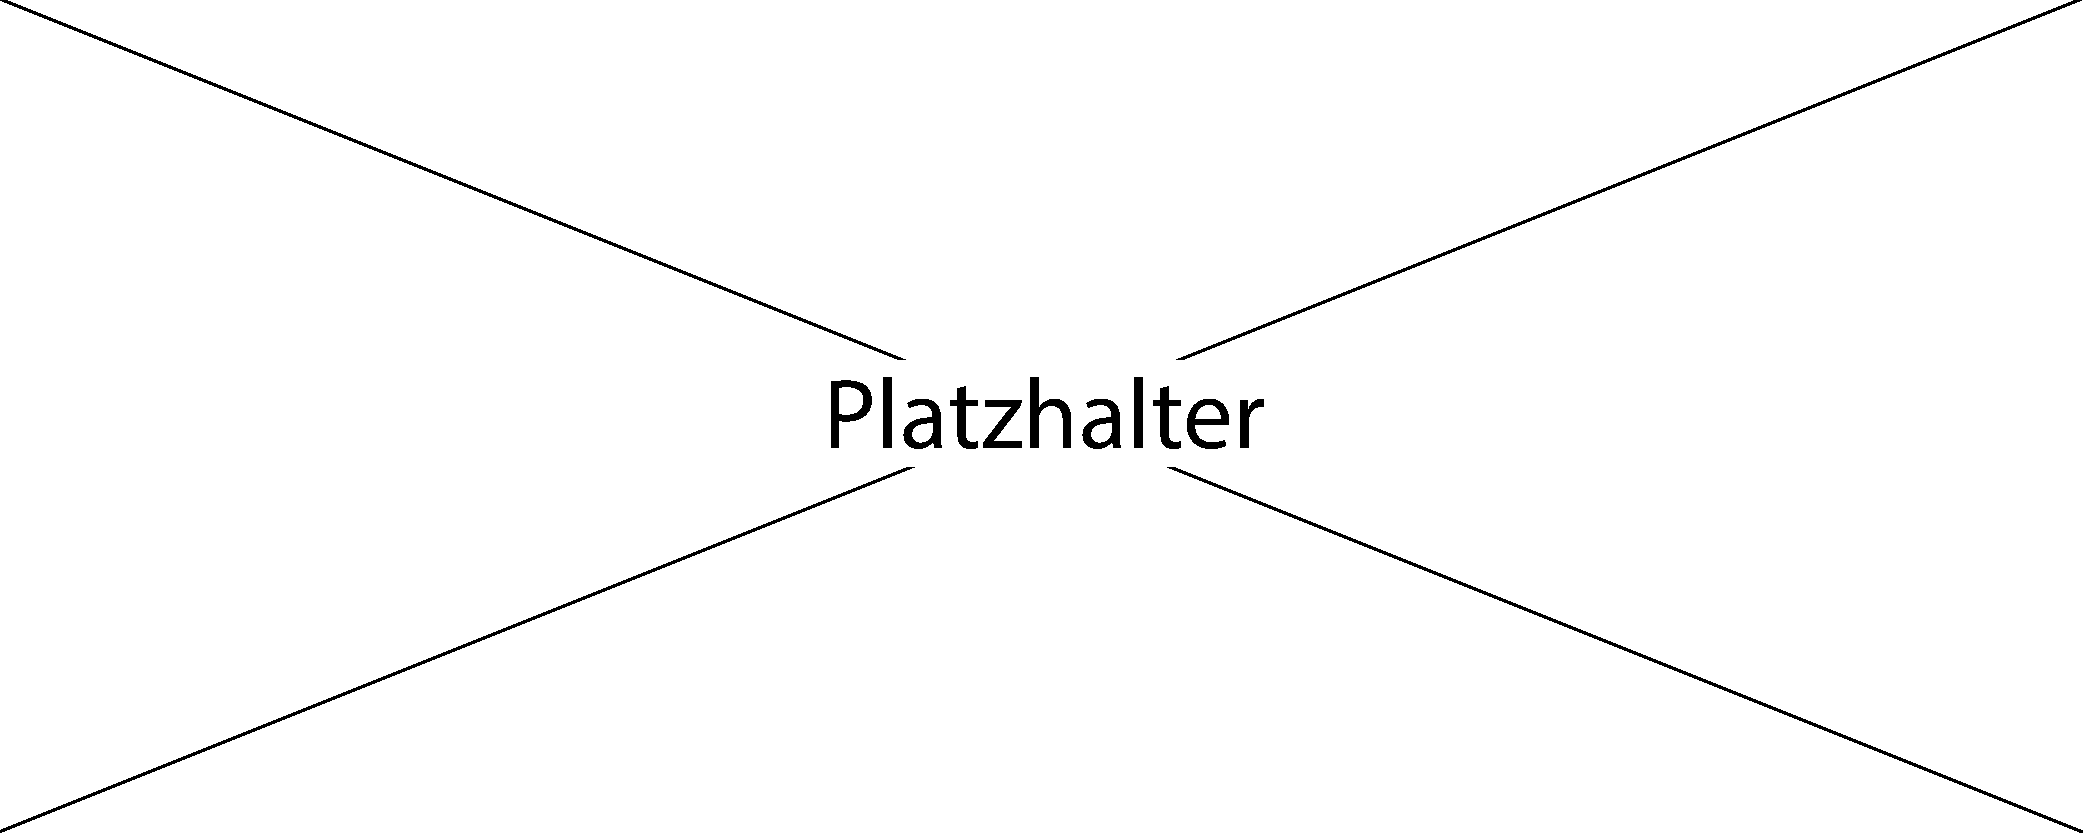
\includegraphics[width=12cm]{figures/sonstiges/platzhalter.pdf}
			\caption{Flowchart des Algorithmus \texttt{RandomSearch}.}
			\label{fig:erg_rs_flow}
		\end{figure}
		Wie darüber hinaus in Abb. \ref{fig:erg_rs_flow} noch einmal verdeutlicht, werden Parameter durch den simplen Input des Rewards variiert und gefunden.\\
		Nach Anwendung der Parametersuche durch \texttt{RandomSearch} wird eine Optimierung des neuronalen Netzes durch den Optimierungsalgorithmus \texttt{Weights} durchgeführt. Die gefundenen Parameter sind unter Umständen noch nicht Perfekt gewählt oder verursachen vereinzelt Probleme, welche die Simulation inkonsistent werden lassen. Bei der Optimierung durch Gewichtung der bestehenden Synapsen könnten nachträglich Parameter beeinflusst und gewisse Wege im neuronalen Netz feiner eingestellt werden. In Abb. \ref{fig:erg_w_flow} wird der gesamte Programmablauf noch einmal verdeutlicht.
		\begin{figure}[!h] %[!t] ...
			\centering
			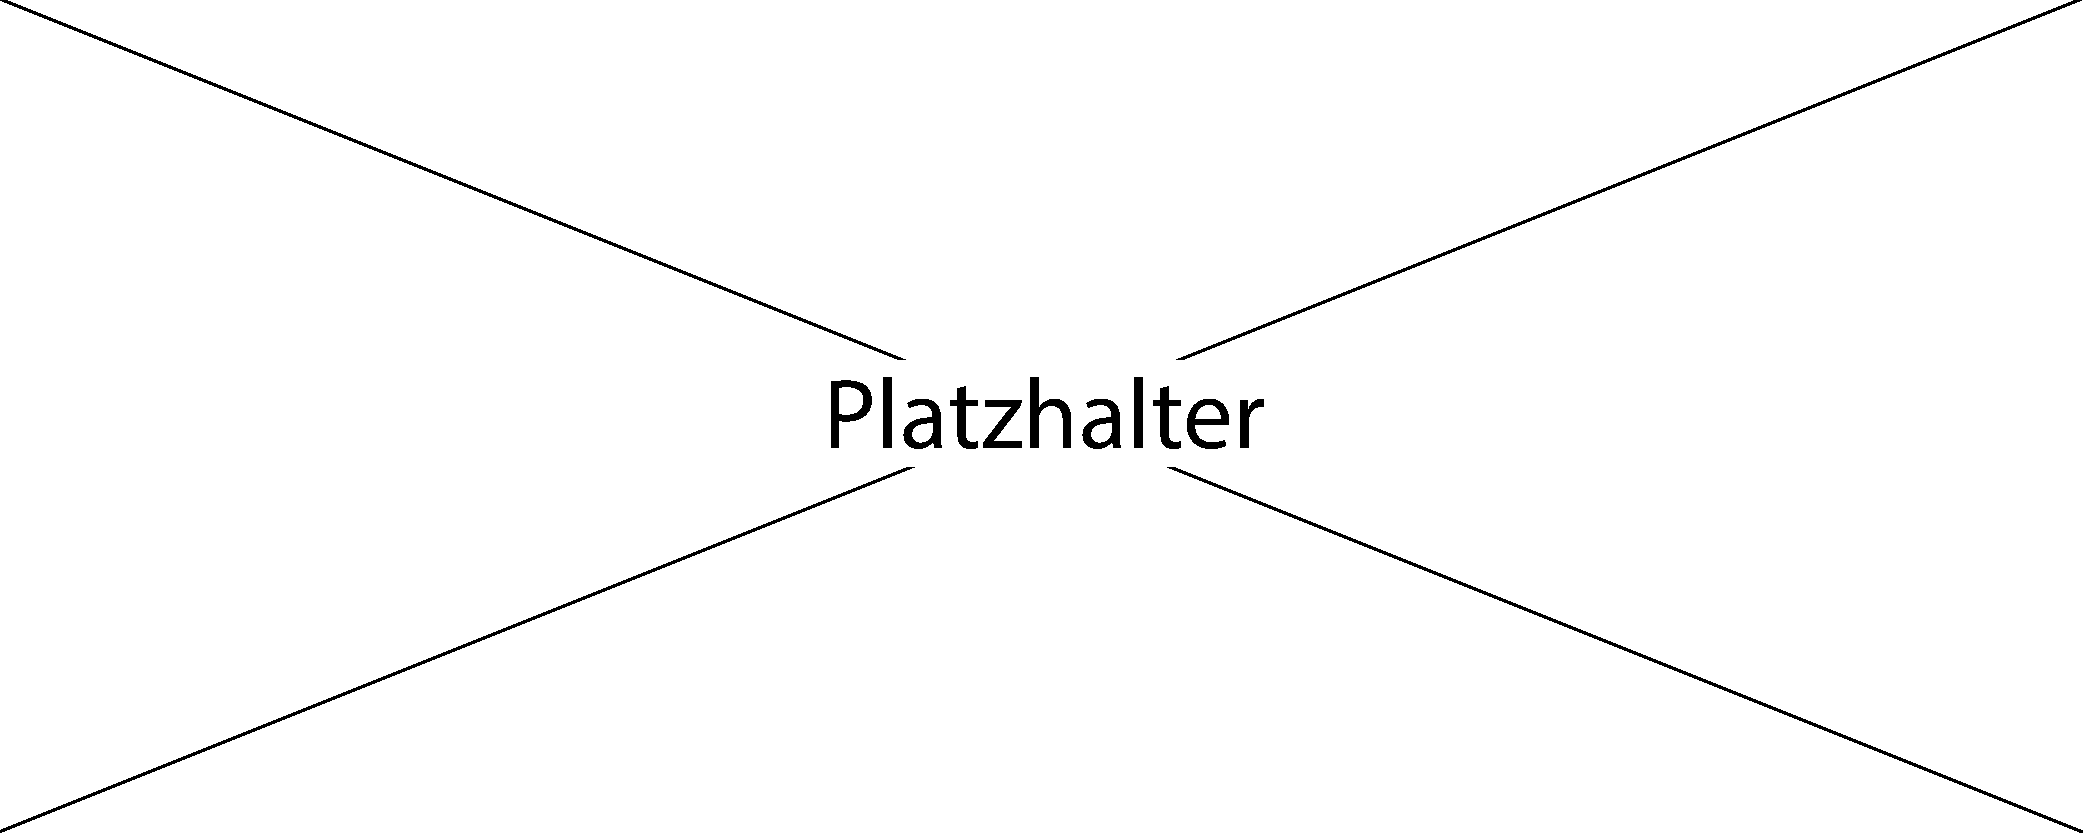
\includegraphics[width=12cm]{figures/sonstiges/platzhalter.pdf}
			\caption{Flowchart des Algorithmus \texttt{Weights}.}
			\label{fig:erg_w_flow}
		\end{figure}
		In Appendix \ref{app:parameter} werden die Ergebnisse der besten Simulationsläufe genauer beschrieben.\\
		Eine weitere Optimierung wurde eingeführt, um das neuronale Netz robuster und effizienter zu gestalten. Anstatt der gesamten 46 Parameter für Nervenzellen Synapsen und Gap-Junctions werden jeweils nur die Hälfte der benötigten Parameter simuliert und anschließend dupliziert. Dies sorgt für eine symmetrische Verteilung von zufällig generierten Parametern und einer noch effizienteren Simulation. Aufgrund der symmetrischen Architektur des gegebenen neuronalen Netzes ist diese Methode zulässig und führt zu sehr guten Ergebnissen.
	\subsection{Alternative Such- und Optimierungsalgorithmen}
		Wie bereits in Sektion \ref{sec:rl_alt} vorgestellt, existieren  viele gute Algorithmen zur Parametersuche und -optimierung von künstlich erzeugten oder gegebenen neuronalen Netzen. Doch die Implementierung dieser Algorithmen besonders auf die hohe Anzahl an zu variierenden Parametern stellt eine hohe Anforderung dar. Klassische Optimierungsverfahren über Kostenfunktionen lassen sich zwar aufstellen (wie in \ref{label}) kurz gezeigt, können aber durch die Anzahl an Nervenzellen, Synapsen und Gap-Junctions nicht weiter optimiert werden.\\
		Einzig die Optimierung durch Gewichtung von Synapsen und Gap-Junctions kann mit bekannten Algorithmen und den Input des Rewards effizienter als durch RandomSearch umgesetzt werden.

% ***
\section{Vergleich zu bestehenden Systemen}
\label{sec:erg_vgl}
% ***
	Vergleich zu bestehenden Systemen aus der Regelungstechnik... tbd

% ***
\section{Zusammenfassung}
\label{sec:erg_zsm}
% ***
	In Zeiten neuer Denkweisen und unkonventioneller Herangehensweisen an bestehende Probleme findet die Anwendung neuronaler Netze und künstlicher Intelligenzen immer mehr Anklang in fast allen Bereichen des Alltags sowie der Wissenschaft. Neue Theorien und Lernalgorithmen lassen hoch parallele Rechenkonstrukte lernen und nutzen diese Methoden, um komplexe Aufgabenstellungen zu lösen. Diese Arbeit untersucht zum einen die Grundzüge des Deep Learning mit Schwerpunkt auf Reinforcement Learning, wendet diese Erkenntnisse jedoch auf unkonventionellem Wege auf bereits bestehende neuronale Netze echter Lebensformen an. Dieser Ansatz wurde noch nicht oft untersucht und bietet eine neue Möglichkeit, von der Evolution zu lernen und besser als bereits bestehende Systeme zu werden.\\
	Dies erfordert jedoch zum einen ein sehr genaues und umfassendes Verständnis von biologischen und chemischen Prozessen in neuronalen Netzen sowie medizinische Grundlagen, zum anderen einen ausgereiften Simulator, welcher diese Prozesse effizient und mit hoher Genauigkeit simulativ nachbilden kann. Darüber hinaus erfordert es gute Lernalgorithmen, um unbekannte Parameter und Assoziationen in neuronalen Netzen zu finden und diese auszubilden.\\
	Prozesse innerhalb neuronaler Netze wurden bereits gut erforscht und dokumentiert. Daher konnte hier auf eine große Wissensdatenbank zurückgegriffen werden, um formulare Zusammenhänge für Größen wie Synapsenströme und Membranpotentiale herzuleiten. Dies ist für den Simulator von großer Bedeutung, da somit die Signalverläufe und Fire-Events dargestellt werden können. Wie anhand der Plots \ref{label} und \ref{label} zu sehen ist, liefert das Leaky Integrate and Fire Modell eine sehr genaue und zuverlässige Simulation der Nervenzellen. Voraussetzung für eine realitätsnahe Simulation sind jedoch stimmige Parameter in jeder einzelnen Nervenzelle und Synapse. Diese Parameter wurden durch Suchalgorithmen und langen Simulationsläufen gefunden und zeigen letztendlich den ursprünglichen Reflex des Wurms C. Elegans: Touch-Withdrawal (zu Deutsch: Rückwärtsbewegung bei Berührung). Weiterhin wurde der Simulator ausgebaut, um ein gegebenes Netzwerk zur Regelung dynamischer Systeme zu nutzen. Auch dies konnte mit Erfolg nachgewiesen werden, wie in Appendix \ref{app:parameter} zu sehen ist.\\
	Zusammenfassend zeigte dieses Thema durch Kombination verschiedener Bereiche der Wissenschaft eine neue Herangehensweise an bereits bestehende Probleme der Regelungstechnik auf. Durch die Aktualität und Neuigkeit der genutzten Werkzeuge und Informationsquellen entstand eine Implementierung, welche durch das Einsetzen des Touch-Withdrawal Neuronal Circuit \cite{WormLevelRL} erfolgreich in der Lage war, dynamische Systeme in der Regelungstechnik zu stabilisieren.\\
	Nichtsdestotrotz gibt es nach wie vor viele Baustellen und Erweiterungsmöglichkeiten.

% ***
\section{Ausblick}
\label{sec:erg_ausblick}
% ***
	Die Anwendung des Reinforcement Learning oder generell des Deep Learning in Bereichen der Regelungstechnik ist noch sehr neu. Besonders der Ansatz, ein existierendes neuronales Netz zur Steuerung dynamischer Systeme zu verwenden wurde in Fachkreisen noch nicht sehr oft dokumentiert. Daher basiert diese Arbeit auf sehr viel Grundlagenforschung zu Nervensystemen des Wurms C.Elegans \cite{CElegans} sowie der Methoden des Reinforcement Learning, um eine Brücke zwischen diesen Themen zu schlagen. Jedoch bietet diese Arbeit gleichzeitig nur ein grundlegendes Verständnis über die Prozesse biologischer neuronaler Netze und dessen Implementierung in einen Simulator.\\
	Schon die Berechnungsmodelle der Synapsenströme und Membranpotentiale sind vereinfacht dargestellt. Wie in dem Buch Neuronal Dynamics \cite{NeuronalDynamics} zu lesen ist, bietet das Leaky Integrate and Fire Modell zwar zeitgenaue und zuverlässige Verhaltenssimulationen der Nervenzellen, hat jedoch an anderen Stellen Nachteile, wie in Sektion \ref{sec:lif_lim} beschrieben.\\
	Weitergehend sollen Parameter und Gewichte für das neuronale Netz gefunden werden, um eine korrekte Simulation und Regelung zu erhalten. Dies ist bisher nur durch die Methode RandomSearch geschehen. Weitere Suchalgorithmen (beschrieben in Sektion \ref{sec:rl_alt}) könnten durch große Anpassungen ebenfalls Anwendung in der Suche nach passenden Parametern finden.\\
	Das Framework des Simulators ist bisher mit dem Projekt gewachsen. Obwohl immer stets auf den universellen und modularen Aufbau geachtet wurde, könnte der Simulator noch allgemeiner implementiert sein und eine größere Anzahl an Funktionen aufweisen. Eine Implementierung als Paket in Python mit Verfügbarkeit über PyPI\footnote{www.pypi.org - Python Package Index} kann ebenfalls möglich sein.	

%%% Local Variables: 
%%% mode: latex
%%% TeX-master: "main"
%%% End: 
